\documentclass{beamer}
\mode<presentation>
\usetheme{CambridgeUS}
\usepackage[russian]{babel}
\usepackage[utf8]{inputenc}
\usepackage[T2A]{fontenc}
\usepackage{sansmathaccent}

\usepackage{verbatim}
\usepackage{alltt}

\pdfmapfile{+sansmathaccent.map}
\title[UX Elements]{Функциональные спецификации и требования к контенту}
\author{Наумов Д.А., доц. каф. КТ}
\date[23.09.2020] {Компьютерная графика и проектирование графических интерфейсов, 2020}

\begin{document}

%ТИТУЛЬНЫЙ СЛАЙД
\begin{frame}
  \titlepage
\end{frame}
  
%СОДЕРЖАНИЕ ЛЕКЦИИ
\begin{frame}
  \frametitle{Содержание лекции}
  \tableofcontents  
\end{frame}

\section{Уровень структуры}
  
\begin{frame}[t]
\begin{block}{Уровень структуры}
третий из пяти уровней. Наши интересы смещаются от абстрактных вопросов стратегии в сторону конкретных факторов, определяющих, что в конечном счете как будет происходить взаимодействие пользователя.
\end{block}
\begin{figure}[h]
\centering
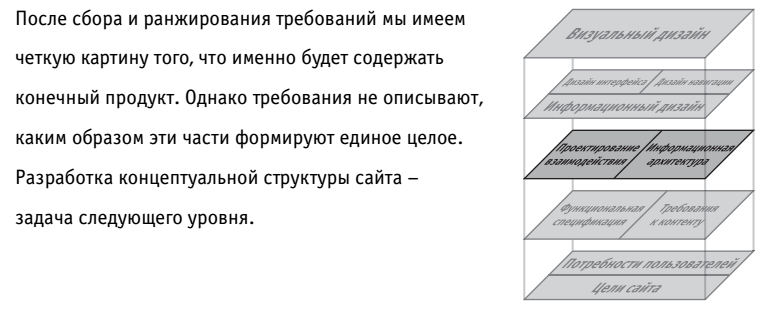
\includegraphics[scale=0.6]{images/lec03-pic01.png}
\end{figure}
\end{frame} 

\begin{frame}[t]
\begin{itemize}
\item В традиционном подходе к разработке программного обеспечения создание структурированного опыта взаимодействия называется проектированием взаимодействия. 
\item В сфере создания контента структурирование опыта взаимодействия – это вопрос информационной архитектуры. 
\end{itemize}
\begin{figure}[h]
\centering
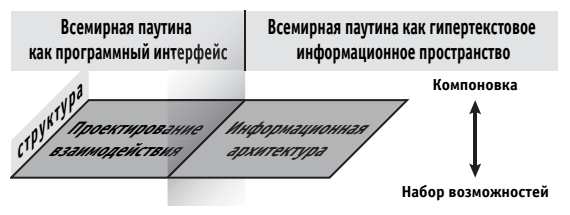
\includegraphics[scale=0.4]{images/lec03-pic02.png}
\end{figure}
Проектирование взаимодействия имеет отношение к реализации возможностей, позволяющих пользователю решать задачи, а информационная архитектура – к реализации возможностей, связанных с предоставлением пользователю информации.
\end{frame} 

\section{Проектирование взаимодействия}

\begin{frame}[t]{Проектирование взаимодействия}
\begin{block}{Концептуальная модель}
собственное представление пользователей о поведении созданных нами интерактивных компонентов. 
\end{block}
\begin{itemize}
	\item корзина с покупками;
	\item форма заказа по каталогу.
\end{itemize}
\end{frame} 

\begin{frame}[t]{Southwest airlines}
\begin{figure}[h]
\centering
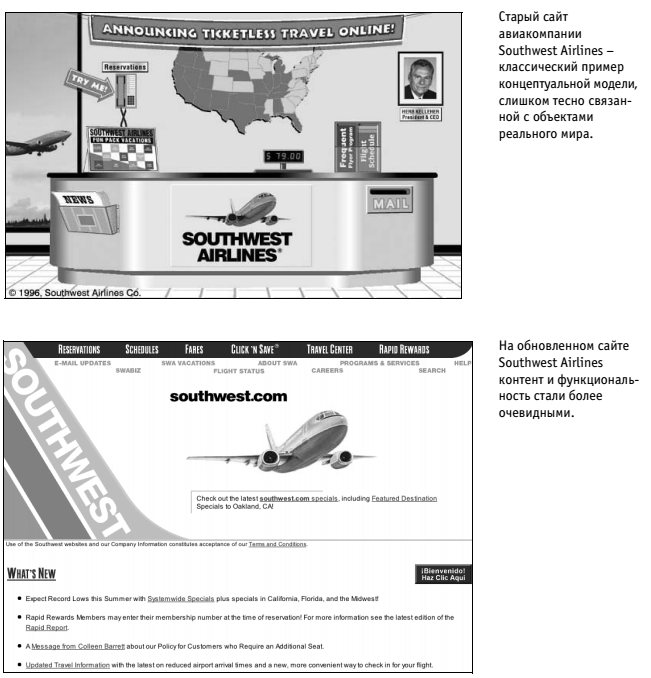
\includegraphics[scale=0.4]{images/lec03-pic03.png}
\end{figure}
\end{frame} 

\begin{frame}[t]{Southwest airlines}
\begin{figure}[h]
\centering
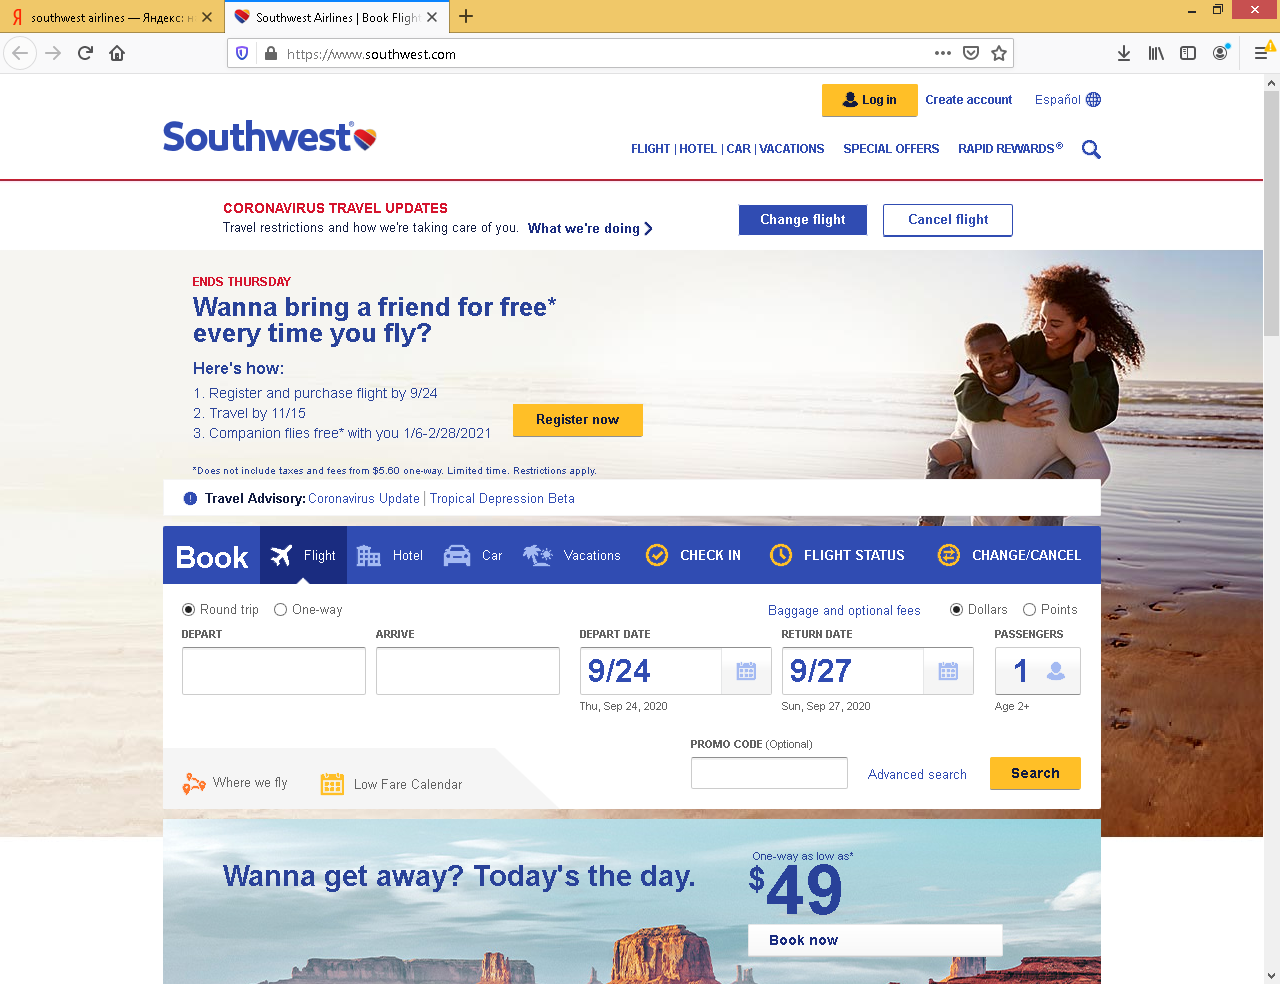
\includegraphics[scale=0.3]{images/lec03-pic04.png}
\end{figure}
\end{frame} 

%\begin{frame}[t]{Southwest airlines}
%\begin{figure}[h]
%\centering
%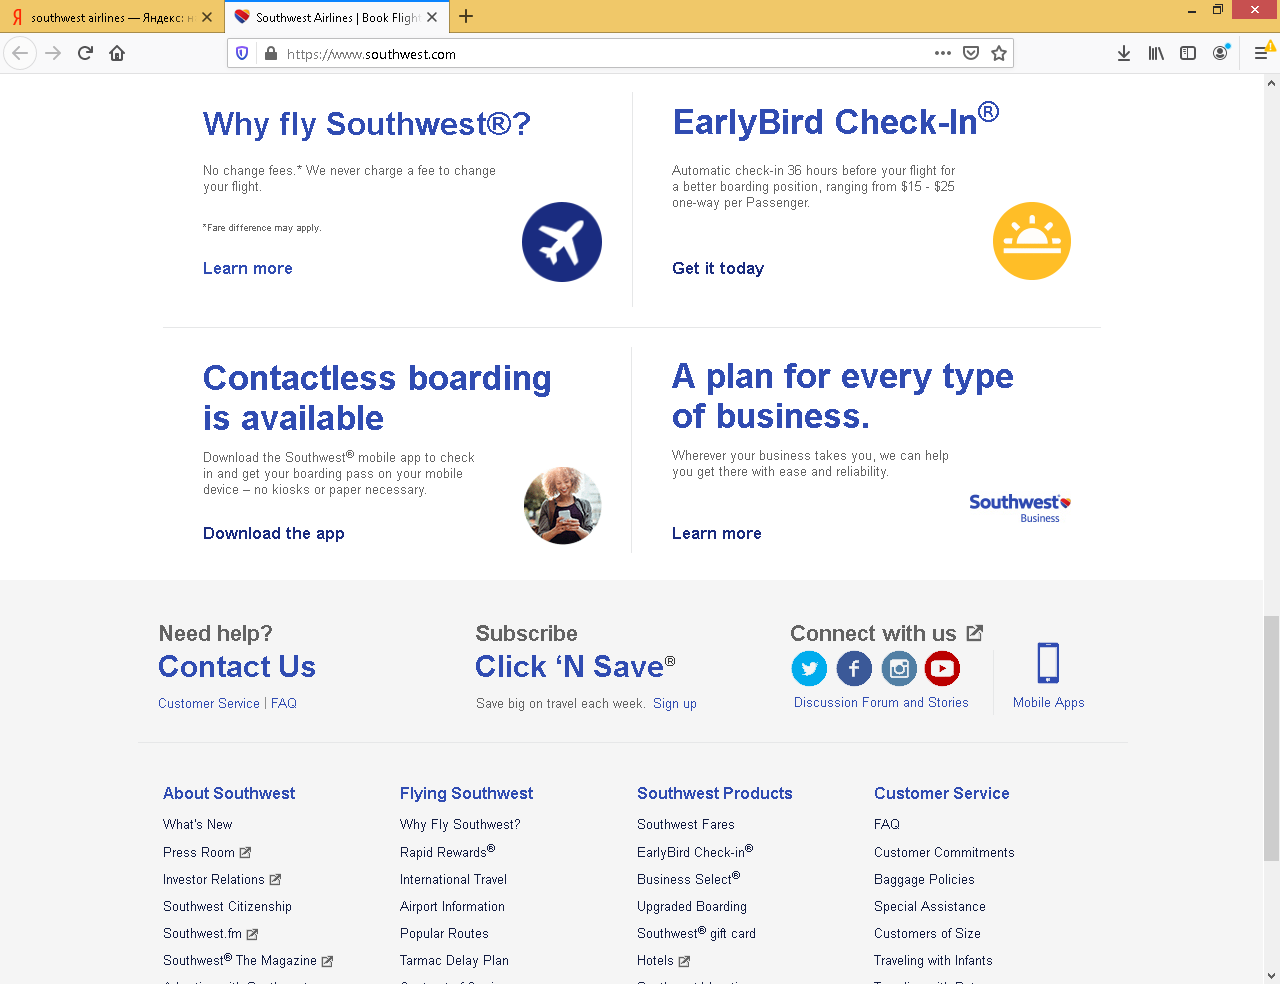
\includegraphics[scale=0.4]{images/lec03-pic05.png}
%\end{figure}
%\end{frame} 

\begin{frame}[t]{Обработка ошибок}
\begin{figure}[h]
\centering
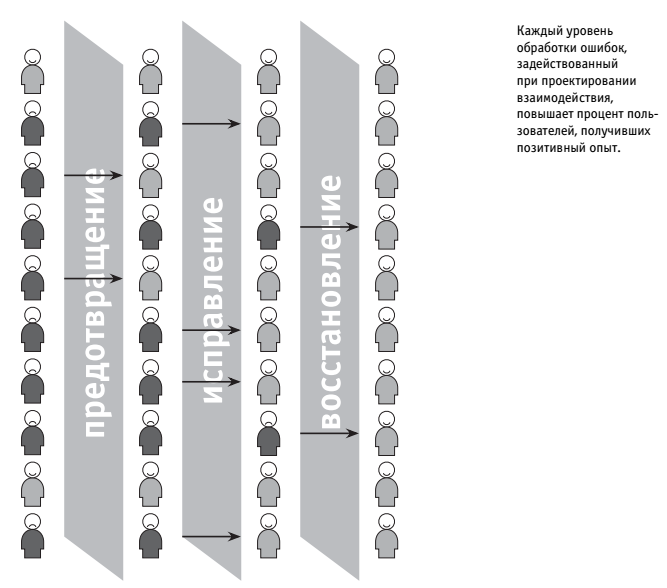
\includegraphics[scale=0.3]{images/lec03-pic06.png}
\end{figure}
\end{frame} 

\section{Информационная архитектура}

\begin{frame}[t]
\textbf{Информационная архитектура} связана с созданием организационных и навигационных схем, обеспечивающих экономичное и эффективное перемещение по сайту. 

~

\textbf{Нисходящий подход} к созданию информационной архитектуры заключается в ее построении непосредственно на основе целей сайта и потребностей пользователей. 
\begin{figure}[h]
\centering
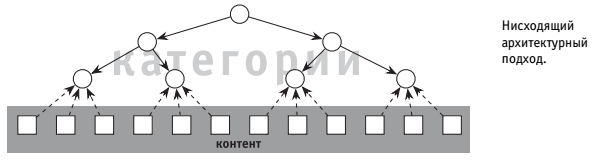
\includegraphics[scale=0.5]{images/lec03-pic07.png}
\end{figure}
\end{frame} 

\begin{frame}[t]
\textbf{Информационная архитектура} связана с созданием организационных и навигационных схем, обеспечивающих экономичное и эффективное перемещение по сайту. 

~

\textbf{Восходящий подход} к построению информационной архитектуры также состоит в выделении категорий и подкатегорий, но при этом в основу ложится анализ контента и функциональных требований. 
\begin{figure}[h]
\centering
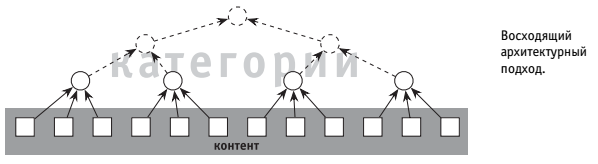
\includegraphics[scale=0.6]{images/lec03-pic08.png}
\end{figure}
\end{frame} 

\begin{frame}[t]{Гибкая архитектура}
\begin{figure}[h]
\centering
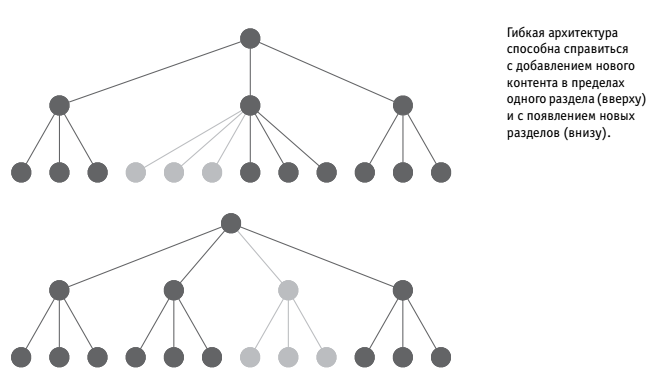
\includegraphics[scale=0.6]{images/lec03-pic09.png}
\end{figure}
\end{frame} 

\begin{frame}[t]{Архитектурные решения}
\begin{figure}[h]
\centering
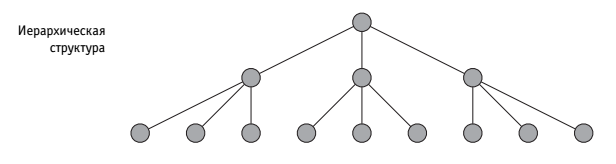
\includegraphics[scale=0.6]{images/lec03-pic10.png}
\end{figure}
\begin{figure}[h]
\centering
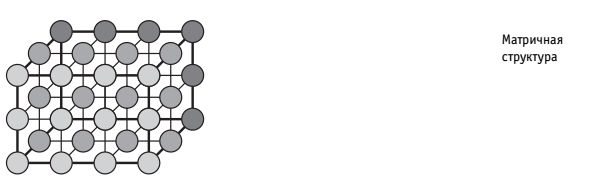
\includegraphics[scale=0.6]{images/lec03-pic11.png}
\end{figure}
\end{frame} 

\begin{frame}[t]{Архитектурные решения}
\begin{figure}[h]
\centering
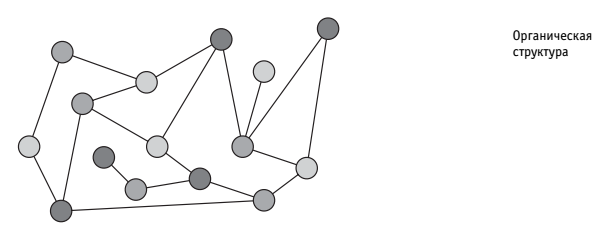
\includegraphics[scale=0.6]{images/lec03-pic12.png}
\end{figure}
\begin{figure}[h]
\centering

\includegraphics[scale=0.6]{images/lec03-pic13.png}
\end{figure}
\end{frame} 

\begin{frame}[t]{Архитектурные решения}
\begin{figure}[h]
\centering
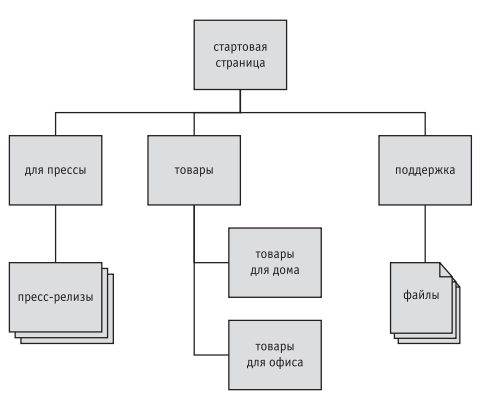
\includegraphics[scale=0.6]{images/lec03-pic14.png}
\end{figure}
\end{frame} 
\begin{frame}{Что читать по данной теме?}
\begin{enumerate}
\item Норманн, Дональд А. «Дизайн привычных вещей». – Пер. с англ. – М.: Вильямс, 2006.
\item Розенфельд Л., Морвиль П. «Информационная архитектура в Интернете», 2-е издание. – СПб.: Символ-Плюс, 2005.
\end{enumerate}
\end{frame}

\section{Информационная архитектура}

\begin{frame}[t]{Навигация главной страницы}
\begin{figure}[h]
\centering
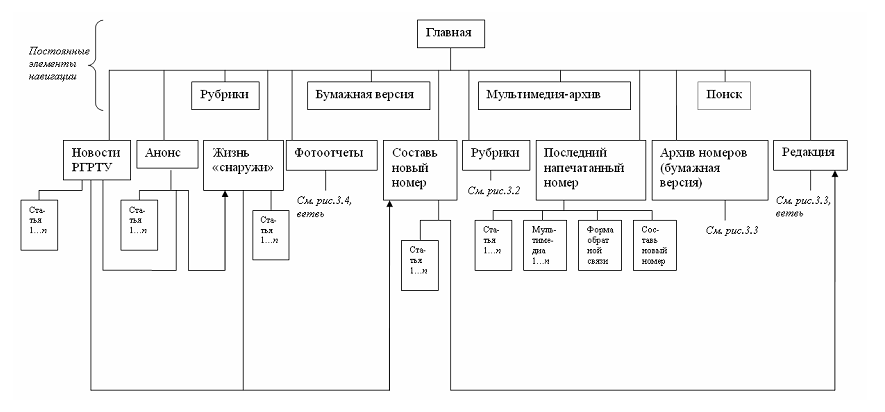
\includegraphics[scale=0.5]{images/lec03-pic15-ex01.png}
\end{figure}
\end{frame}

\begin{frame}[t]{Навигация страниц рубрик}
\begin{figure}[h]
\centering
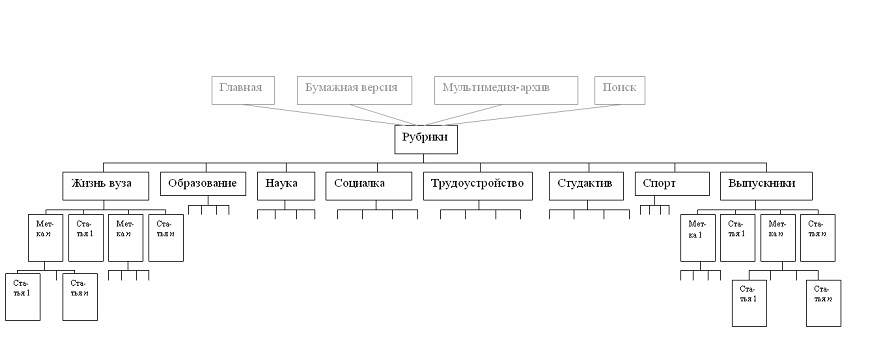
\includegraphics[scale=0.5]{images/lec03-pic15-ex02.png}
\end{figure}
\end{frame}

\begin{frame}[t]{Навигация страницы бумажная версия}
\begin{figure}[h]
\centering
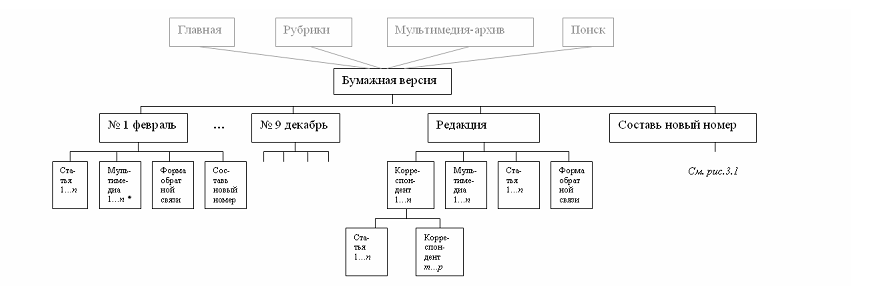
\includegraphics[scale=0.5]{images/lec03-pic15-ex03.png}
\end{figure}
\end{frame}

\begin{frame}[t]{Навигация страницы мультимедиа-архив}
\begin{figure}[h]
\centering
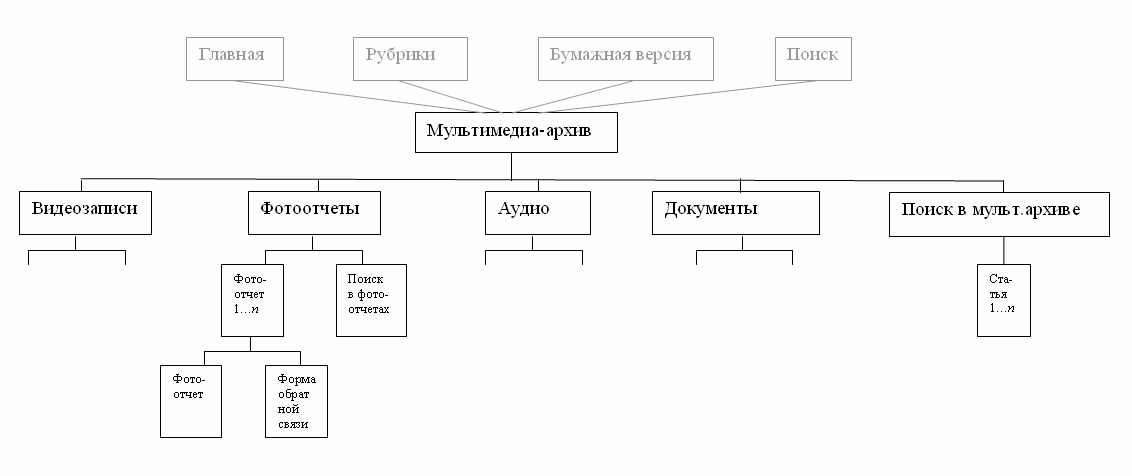
\includegraphics[scale=0.4]{images/lec03-pic15-ex04.png}
\end{figure}
\end{frame}

\end{document}
